\documentclass{report}
\usepackage[utf8]{inputenc}
\usepackage[x11names]{xcolor}

\usepackage{listings}
%%\usepackage{listingsutf8}
%%\lstset{inputencoding=utf8/latin1}

\renewcommand{\lstlistingname}{Programa}
\renewcommand{\lstlistlistingname}{Índice de programas}


\usepackage{tikz}
\usetikzlibrary{arrows.meta}
\usetikzlibrary{decorations.pathreplacing}
\newcommand*{\tikzgrid}[2]{\draw[help lines](0,0)grid[step=0.2,lightgray,ultra thin](#1,#2);\draw[help lines](0,0)grid[gray](#1,#2);\foreach\x in{0,1,...,#1}\node[below]at(\x,0){\scriptsize\x};\foreach\y in{1,2,...,#2}\node[left]at(0,\y){\scriptsize\y};}


\usepackage[linktocpage=true, breaklinks=true,colorlinks=true, urlcolor=-DarkOrchid1, pdfstartview=FitH]{hyperref}


\begin{document}


\tikz{\draw(0,0)rectangle(2mm,2mm);}

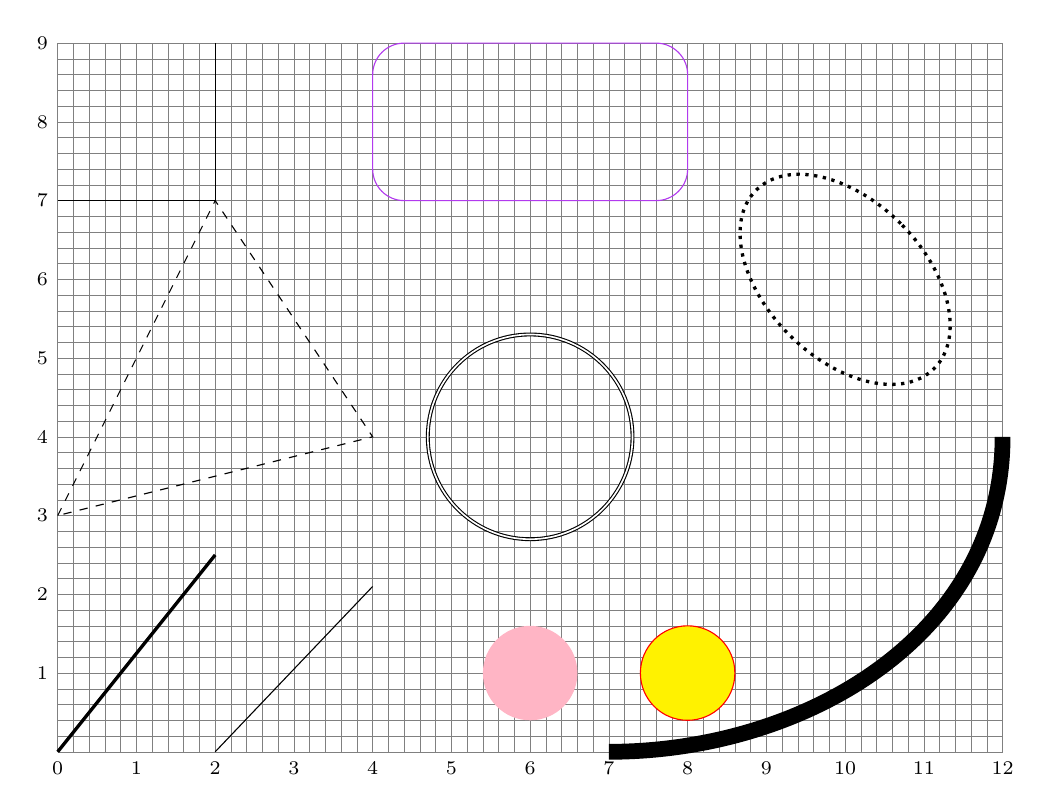
\begin{tikzpicture}
\tikzgrid{12}{9}
\path[draw,very thick](0,0)--(2,2.5);
\draw(2,0)--(4,2.1);
\draw[dashed](0,3)--(2,7)--(4,4)--cycle;
\draw(0,7)-|(2,9);
\draw[rounded corners=4mm,DarkOrchid2](4,7)rectangle(8,9);
\draw[double](6,4)circle[radius=1.3cm];
\draw[dotted,very thick](10,6)circle[x radius=1cm,y radius=1.6cm,rotate=45];
\draw[line width=2mm](7,0)to[out=0,in=270](12,4);
\fill[Pink1](6,1)circle[radius=6mm];
\filldraw[color=yellow,draw=red](8,1)circle[radius=6mm];
\end{tikzpicture}

\begin{figure}[!h]
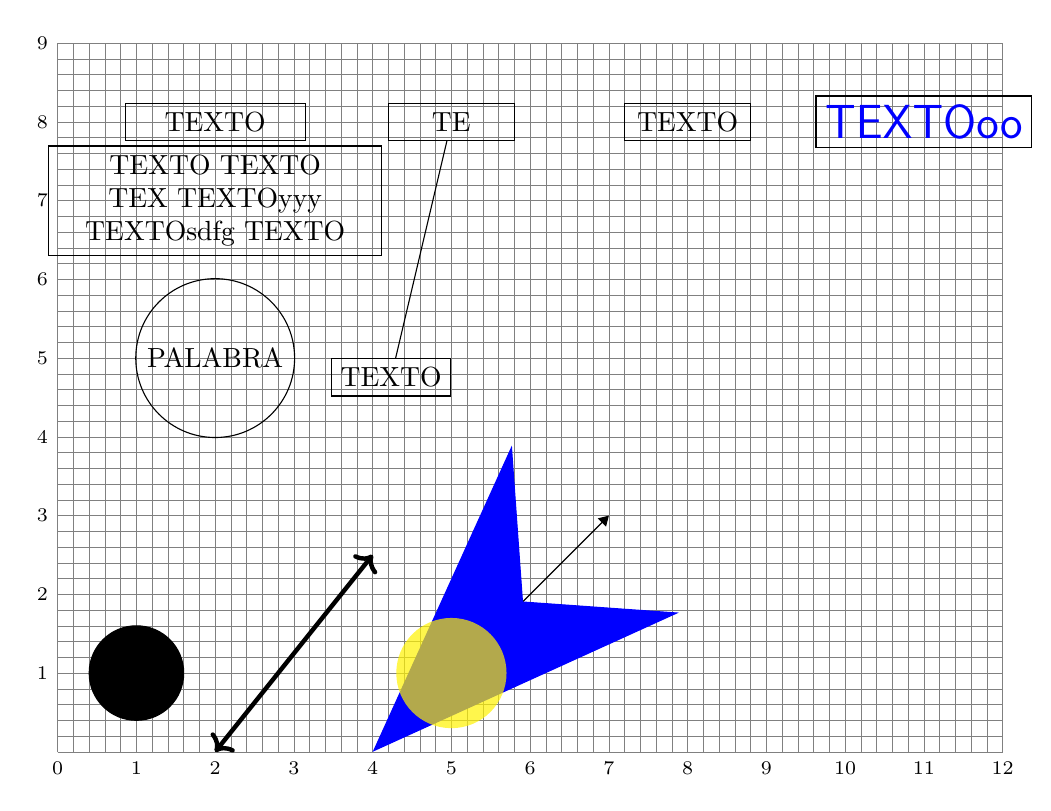
\begin{tikzpicture}
\tikzgrid{12}{9}
\useasboundingbox(0,0)rectangle(12,9);
\filldraw(1,1)circle[radius=6mm];
\draw[ultra thick,arrows=<->](2,0)--(4,2.5);
\draw[arrows={Stealth[scale=5,blue, length=8mm]}-Triangle](4,0)--(7,3);
\fill[yellow,opacity=0.7](5,1)circle[radius=7mm];
\node[draw,shape=circle] at(2,5){PALABRA};
\node[draw,inner xsep=5mm]at(2,8){TEXTO};
\node[draw,minimum width=16mm](AA)at(5,8){TE};
\node[draw,minimum width=16mm]at(8,8){TEXTO};
\node[draw,minimum width=16mm,text=blue, font=\sffamily\LARGE]at(11,8){TEXTOoo};
\node[draw,text width=4cm,align=center] at(2,7){ TEXTO TEXTO TEX TEXTOyyy TEXTOsdfg TEXTO};
\node[draw,below left](FF)at(5,5){TEXTO};
\draw(AA)--(FF);
\end{tikzpicture}
\caption{mi figura en tikz}
\end{figure}

\clearpage

\begin{tikzpicture}
%\tikzgrid{6}{6}
\draw[arrows=->,thick](-5,0)--(5,0);
\draw[arrows=->,thick](0,-5)--(0,5);
\draw[domain=-3:3] plot(\x,\x);
\draw[domain=0.11:3,samples=100,smooth]plot(\x,{ln(\x)});
\draw[blue,domain=-3:3]plot(\x,{sin(\x r)});
\end{tikzpicture}

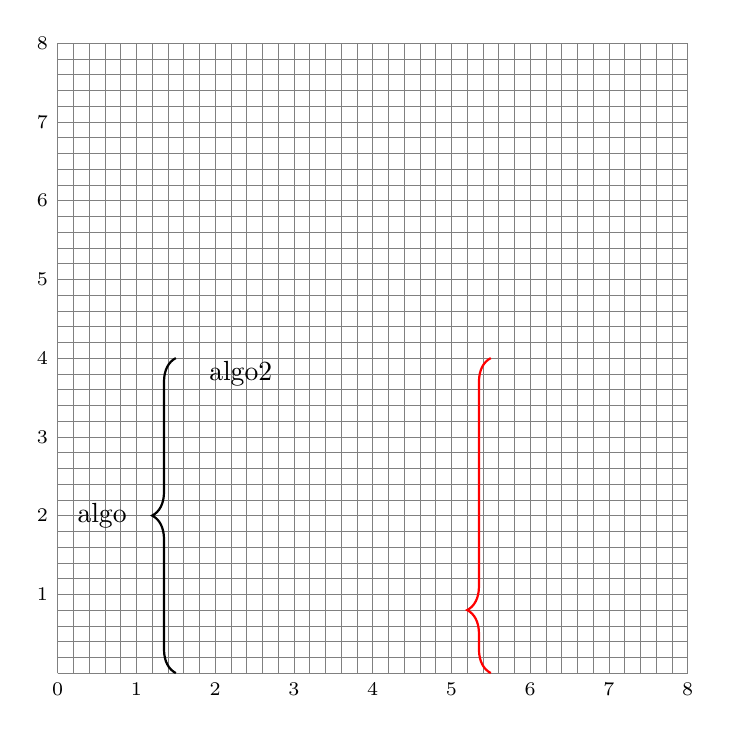
\begin{tikzpicture}
\tikzgrid{8}{8}
\draw[thick,decoration={brace,amplitude=3mm}, decorate](1.5,0)--(1.5,4);
\node[left] at(1,2){algo};
\node[right]at(1.8,3.8){algo2};
\draw[red,thick,decoration={brace, amplitude=3mm,aspect=0.2}, decorate](5.5,0)--(5.5,4);
\end{tikzpicture}










\newpage



\tableofcontents

%\lstlistoflistings

\chapter{Aprendiendo a poner programas \texorpdfstring{$\int$}{integral}}

\href{http://www.uni.edu.pe}{Universidad}


\hyperlink{fin}{final del documento}
\hypertarget{inicio}{i}

\ \\[2cm]


\url{http://www.uni.edu.pe}

\url{https://www.google.com.pe/search?q=uni&oq=uni&aqs=chrome..69i57j0l5.559j0j8&sourceid=chrome&ie=UTF-8}

\section{algo fácil}

texto texto \lstinline|\end{document}| texto texto

\begin{lstlisting}
  \huge
  \textbf{ }
  For 
  If
\end{lstlisting}

%%\lstinputlisting{picins2.sty}
%%\lstinputlisting{picins.sty}

texto texto2 texto3

\begin{lstlisting}[float=h,aboveskip=3cm]
#include <stdio.h>
int main()
{
    int number;

    printf("Enter an integer: ");
    scanf("%d", &number);

    // True if the number is perfectly divisible by 2
    if(number % 2 == 0)
        printf("%d is even.", number);
    else
        printf("%d is odd.", number);

    return 0;
}
\end{lstlisting}


texto texto2


\begin{lstlisting}[firstline=6, lastline=9]
#include <stdio.h>
int main()
{
    int number;

    printf("Enter an integer: ");
    scanf("%d", &number);

    // True if the number is perfectly divisible by 2
    if(number % 2 == 0)
        printf("%d is even.", number);
    else
        printf("%d is odd.", number);

    return 0;
}
\end{lstlisting}

\begin{lstlisting}[linerange={6-10}]
#include <stdio.h>
int main()
{
    int number;

    printf("Enter an integer: ");
    scanf("%d", &number);

    // True if the number is perfectly divisible by 2
    if(number % 2 == 0)
        printf("%d is even.", number);
    else
        printf("%d is odd.", number);

    return 0;
}
\end{lstlisting}

\section{intermedio}

\begin{lstlisting}[gobble=8]
#include <stdio.h>
int main()
{
    int number;

    printf("Enter an integer: ");
    scanf("%d", &number);

    // True if the number is perfectly divisible by 2
    if(number % 2 == 0)
        printf("%d is even.", number);
    else
        printf("%d is odd.", number);

    return 0;
}
\end{lstlisting}



\lstinputlisting[linerange={30-50}, language=TeX]{picins.sty}

\begin{lstlisting}[language=C, basicstyle=\ttfamily\Large]
#include <stdio.h>
int main()
{
    int number;

    printf("Enter an integer: ");
    scanf("%d", &number);

    // True if the number is perfectly divisible by 2
    if(number % 2 == 0)
        printf("%d is even.", number);
    else
        printf("%d is odd.", number);

    return 0;
}
\end{lstlisting}


\begin{lstlisting}[showtabs=true, showspaces=true]
#include <stdio.h>
int main()
{
    int number;

    printf("Enter an integer: ");
    scanf("%d", &number);

    // True if the number is perfectly divisible by 2
    if(number % 2 == 0)
        printf("%d is even.", number);
    else
        printf("%d is odd.", number);

    return 0;
}
\end{lstlisting}

\begin{lstlisting}[numbers=left,
numberstyle={\scriptsize\color{blue!25}}, numberblanklines=false]
#include <stdio.h>
int main()
{
    int number;

    printf("Enter an integer: ");
    scanf("%d", &number);

    // True if the number is perfectly divisible by 2
    if(number % 2 == 0)
        printf("%d is even.", number);
    else
        printf("%d is odd.", number);

    return 0;
}
\end{lstlisting}

\section{avanzado}

\begin{lstlisting}[numbers=left,
numberstyle={\scriptsize\color{blue!25}}, numberblanklines=false,firstline=10, firstnumber=10]
#include <stdio.h>
int main()
{
    int number;

    printf("Enter an integer: ");
    scanf("%d", &number);

    // True if the number is perfectly divisible by 2
    if(number % 2 == 0)
        printf("%d is even.", number);
    else
        printf("%d is odd.", number);

    return 0;
}
\end{lstlisting}

\begin{lstlisting}[caption={Mi primer programa pirateado}]
#include <stdio.h>
int main()
{
    int number;

    printf("Enter an integer: ");
    scanf("%d", &number);

    // True if the number is perfectly divisible by 2
    if(number % 2 == 0)
        printf("%d is even.", number);
    else
        printf("%d is odd.", number);

    return 0;
}
\end{lstlisting}

\lstinputlisting[linerange={30-50}, language=TeX, caption={copiado de CTAN}, label={pro1},captionpos=b]{picins.sty}


Usando el programa \ref{pro1} se aprende a poner gráficos al lado de texto





\begin{lstlisting}[linewidth=8cm, breaklines= true]
#include <stdio.h>
int main()
{
    int number;

    printf("Enter an integer: ");
    scanf("%d", &number);

    // True if the number is perfectly divisible by 2
    if(number % 2 == 0)
        printf("%d is even.", number);
    else
        printf("%d is odd.", number);

    return 0;
}
\end{lstlisting}

\begin{lstlisting}[xleftmargin=5cm]
#include <stdio.h>
int main()
{
    int number;

    printf("Enter an integer: ");
    scanf("%d", &number);

    // True if the number is perfectly divisible by 2
    if(number % 2 == 0)
        printf("%d is even.", number);
    else
        printf("%d is odd.", number);

    return 0;
}
\end{lstlisting}

\begin{lstlisting}[frame=single, framerule=2pt, backgroundcolor=\color{yellow!40}, rulecolor=\color{red}]
#include <stdio.h>
int main()
{
    int number;

    printf("Enter an integer: ");
    scanf("%d", &number);

    // True if the number is perfectly divisible by 2
    if(number % 2 == 0)
        printf("%d is even.", number);
    else
        printf("%d is odd.", number);

    return 0;
}
\end{lstlisting}

\begin{lstlisting}[mathescape=true]
  integral $\int_a^b$
\end{lstlisting}

\begin{lstlisting}[escapechar=|]
  hola mec|á|nica
\end{lstlisting}

\begin{lstlisting}[inputencoding=utf8, literate={á}{{\'a}}1{é}{{\'e}}1{ñ}{{\~n}}1]

mecánica té ñandu
\end{lstlisting}














\newpage

\begin{verbatim}
       hola      mundo


  hoy     dia
\end{verbatim}

\hypertarget{fin}{Mifinal}
\hyperlink{inicio}{inicio del doc}

\end{document}